%%%%%%%%%%%%%%%%%%%%%%%%%%%%%%%%%%%
\subsection{Thermometers}
\label{sec:fdgen-slow-cryo-therm}
% anselmo, jelena,

A detailed \threed temperature map is important to monitor the correct functioning of the cryogenics system and the \lar uniformity.
Given the complexity and size of purity monitors, those can only be installed on the cryostat sides to provide a local measurement of
the \lar purity. While a direct measurement of the \lar purity across the entire cryostat is not viable, a sufficiently detailed \threed temperature map
can be used to predict the \lar purity using \dword{cfd} simulations. Measuring the vertical temperature profile is especially important since this is closely related to
the \lar recirculation and uniformity. 

High-precision temperature sensors are distributed near the TPC walls in two ways:
(1) in high-density (\(>2\) sensors/\si{m}) vertical arrays (the T-gradient monitors), and (2) in coarser ($\sim$ 1 sensor/\SI{5}{m}) \twod arrays 
at the top and bottom of the detector, which are the most sensitive regions (the individual sensors).   

Since temperature variations inside the cryostat are expected to be very small ($\SI{0.02}{K}$, see Figure~\ref{fig:cfd-example}), to properly measure the \threed temperature map 
sensors must be cross-calibrated to better than $\SI{0.005}{K}$. Most sensors are calibrated in the laboratory, prior to installation,
as described in Section~\ref{sp-cisc-thermom-static-t}.  This is in fact the only viable method for sensors in areas where the available space is restricted: on the long sides of the detector
(behind the \dwords{apa} for SP, and behind the lateral %FC end-walls 
\dword{ewfc} for \dual) and top/bottom of the detector.
Given the precision required and the unknown longevity of the sensors (which could require a new calibration after some time), a complementary method
is used for T-gradient monitors behind the front endwalls, at least for the \dword{spmod}.
In those areas there is sufficient space for a movable system that can be used to cross-calibrate in situ
the temperature sensors. %This calibration method is described in the section about dynamic T-gradient monitors. 

In the baseline design for all three systems mentioned above, three elements are common: sensors, cables and readout system.
Platinum sensors with \SI{100}{\ohm} resistance, PT100 series, produced by Lakeshore\footnote{Lakeshore\texttrademark{}, \url{https://www.lakeshore.com/Pages/Home.aspx}.},
are adequate for the temperature range of interest, \SIrange{83}{92}{K}, since in this range those sensors have high reproducibility 
$\sim\SI{5}{mK}$ and absolute temperature accuracy of \SI{100}{mK}.
In addition, the plan is to use the four-wire readout, greatly reducing the issues related to the lead resistance, any parasitic resistances,
connections through the flange, and general electromagnetic noise pick-up. The Lakeshore PT102 sensors
%(see Figure~\ref{fig:sensor_cable}-Left)
have being previously used in the \dword{35t} and \dword{pdsp} detector,
giving excellent results. For the inner readout cables a custom cable made by Axon~\footnote{Axon\texttrademark{}, \url{http://www.axon-cable.com/en/00_home/00_start/00/index.aspx}} is the baseline. It consists in four teflon-jacketed 
cupper wires (AWG28), forming two twisted pairs, with an metallic external shield
and an outer teflon jacket.
%Further details are given in Figure~\ref{fig:sensor_cable}-Right. 
The readout system is described below in  Section~\ref{sec:fdgen-slow-cryo-therm-readout}. %a separate subsection. 

%As shown in Figure~\ref{fig:sensor_cable}, the PT102 sensor has a length of \SI{21}{mm}, which can easily be accommodated in the DUNE T-gradient monitors. 

%\begin{dunefigure}[DUNE baseline choices for sensor and cable]{fig:sensor_cable}
%  {DUNE baseline choices for sensor and cable. Left: Schematic diagram of the PT102 sensor from the Lakeshore company. Right: Schematic diagram and properties of the four wires cable from the
%  Axon company}
%  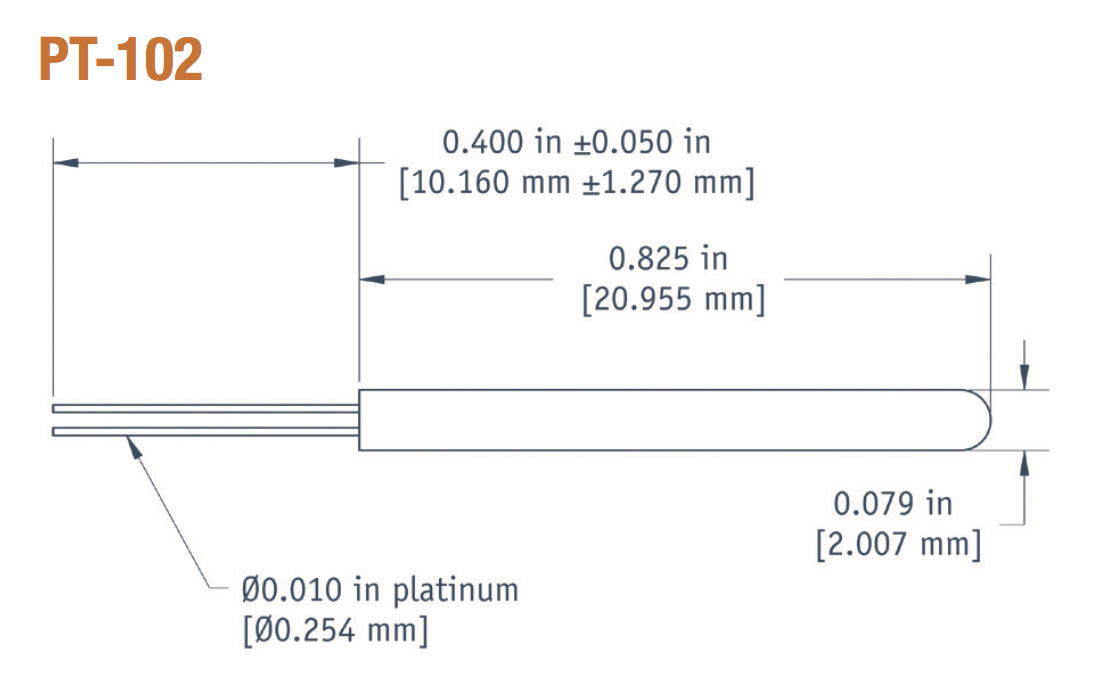
\includegraphics[width=0.4\textwidth]{cisc_pt102.png}
%  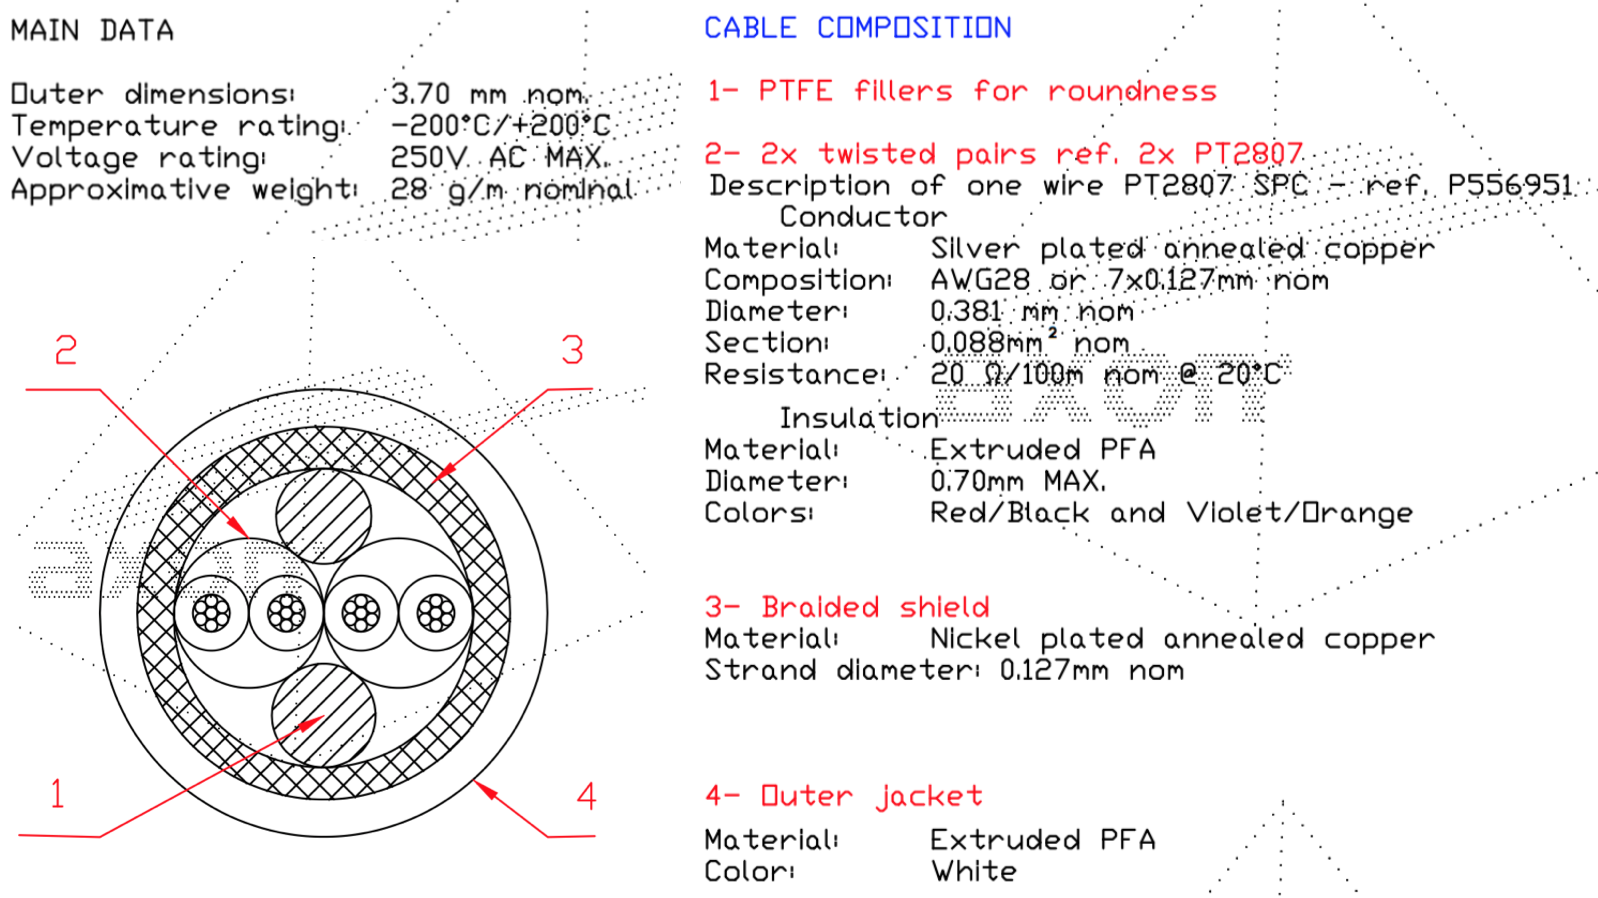
\includegraphics[width=0.55\textwidth]{cisc_TAxonCable.png}
%\end{dunefigure}

Another set of lower-precision sensors is used to monitor the filling of the cryostat in its initial stage. Those sensors are epoxied into the cryostat bottom membrane with
a density to be determined, not to exceed one sensor every \SI{5}{m}. 
Finally, the inner walls and roof of the cryostat are instrumented with the same type of sensors in order to monitor their temperature during cooldown and filling.
The baseline distribution has three vertical arrays of sensors epoxied to the membrane: one behind each of the two %FC front end-walls 
front \dwords{ewfc} and the third one in the middle of the cryostat
(behind the \dwords{apa} for \single and behind the lateral %FC end-walls 
\dwords{ewfc} for \dual). 

%except for the membrane sensors that may come from Minco.

% % % %
\subsubsection{Static T-gradient Monitors}
\label{sp-cisc-thermom-static-t}

Several vertical arrays of high-precision temperature sensors cross-calibrated in the laboratory are installed near the lateral walls
(behind the \dwords{apa} for \single and behind the lateral %FC end-walls 
\dwords{ewfc} for \dual). 
For the \dword{spmod}, since the electric potential is zero behind the \dwords{apa}, no \efield shielding is required, simplifying enormously the mechanical design.
This does not apply for the \dword{dpmod}, for which the proper shielding must be provided. 


Sensors are cross-calibrated in the lab using a well controlled environment and a high-precision readout system, described below in Section~\ref{sec:fdgen-slow-cryo-therm-readout}. %a separate subsection.
Although the calibration procedure will certainly improve, the one currently used for \dword{pdsp} is described here.
Four sensors are placed as close as possible (such that identical temperature can be assumed for all of them) inside a small cylindrical aluminum capsule,
which protects the sensors from thermal shocks and helps in minimizing convection.
One of the sensors acts as reference while the other three are %the ones being 
calibrated. Five independent calibrations
are performed for each set of three sensors, such that the reproducibility of each sensor can be computed. For each calibration 
the capsule is introduced in a PLA box of size \(9.5\times9.5\times\SI{19}{cm^3}\), with two concentrical independent volumes of \lar
and surrounded by a polystyrene box with \SI{15}{cm} thick walls. A small quantity of \lar is used to slowly
cool down the capsule to $\sim\SI{90}{K}$, avoiding thermal shocks that could damage the sensors.
Then the capsule is covered by
\fixme{immersed in?}  \lar such that it penetrates
inside, fully covering the sensors. Once the temperature stabilizes to the 1-\SI{2}{mK} level (after 5-15 minutes) measurements are taken. Then the capsule is taken out from \lar
and kept at room temperature until it reaches \SI{200}{K}. As mentioned above, this procedure is repeated five times, before going to the next set of three sensors.  
As shown in Figure~\ref{fig:Trepro} a reproducibility (\rms of the mean offset in the flat region) of $\sim \SI{2}{mK}$ has been achieved in the \dword{pdsp} design.  

%The baseline design for the mechanics of the system is shown in Figure~\ref{}. It consists in two stainless strings anchored at top and bottom corners of the cryostat
The baseline design for the mechanics of the \single system consists in two stainless strings anchored at top and bottom corners of the cryostat
using the available M10 bolts (see Figure~\ref{fig:sensor-support}-Left). One of the strings is used to route the cables while the other,
separated \SI{340}{mm}, serves as support for temperature sensors.
Given the height of the cryostat, the need of intermediate anchoring points is under discussion. For the \dword{dpmod} no baseline design exists yet,
since additional complications due to the required \efield shielding must be taken into account. Figure~\ref{fig:sensor-support}-Right shows baseline design of the
PCB support for temperature sensors, with an IDC-4 male connector. It has a size of $52\times \SI{15}{mm^2}$. Each four-wire cable from the sensor to the flange has an IDC-4 female connector
on the sensor side; on the other side, it is directly soldered into the inner pins of male SUBD-25 connectors on the flanges. The CF63 side ports on \dword{dss}/cryogenic ports are 
%which will be 
used to extract the cables. 

\begin{dunefigure}[Cryostat bolts and temperature sensor support]{fig:sensor-support}
  {Left: bolts at the bottom corner of the cryostat. Right: Lakeshore PT102 sensor mounted on a PCB with an IDC-4 connector.}
  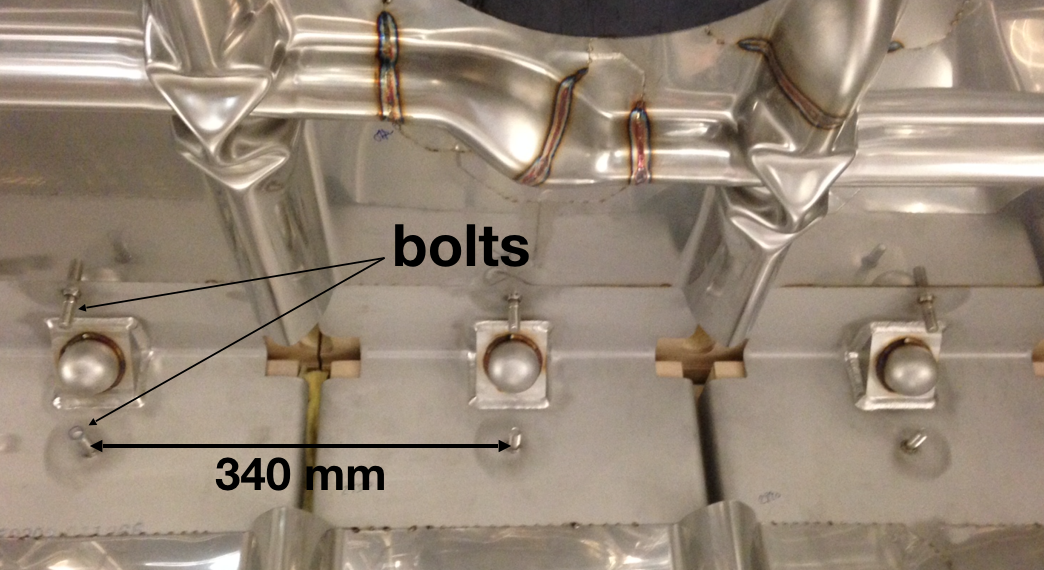
\includegraphics[height=0.2\textwidth]{cisc_cryostat_bolts.png}%
    \hspace{1cm}%
  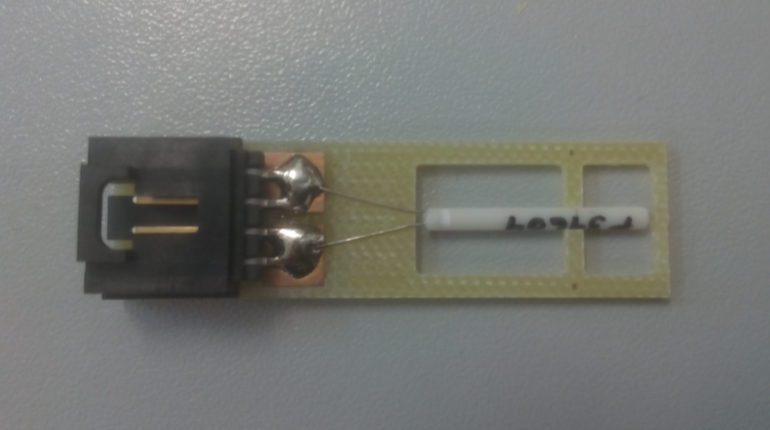
\includegraphics[height=0.2\textwidth]{cisc_tsensor.png}%
\end{dunefigure}


\begin{dunefigure}[Temperature sensor resolution and reproducibility]{fig:Trepro}
  {Temperature offset between two sensors as a function of time for five independent inmersions in \lar. The reproducibility of those sensors,
    defined as the RMS of the mean offset in the flat region, is $\sim \SI{2}{mK}$,
    The resolution for individual measurements, defined as the RMS of one of the offsets in the flat region, is better than \SI{1}{mK}.}
  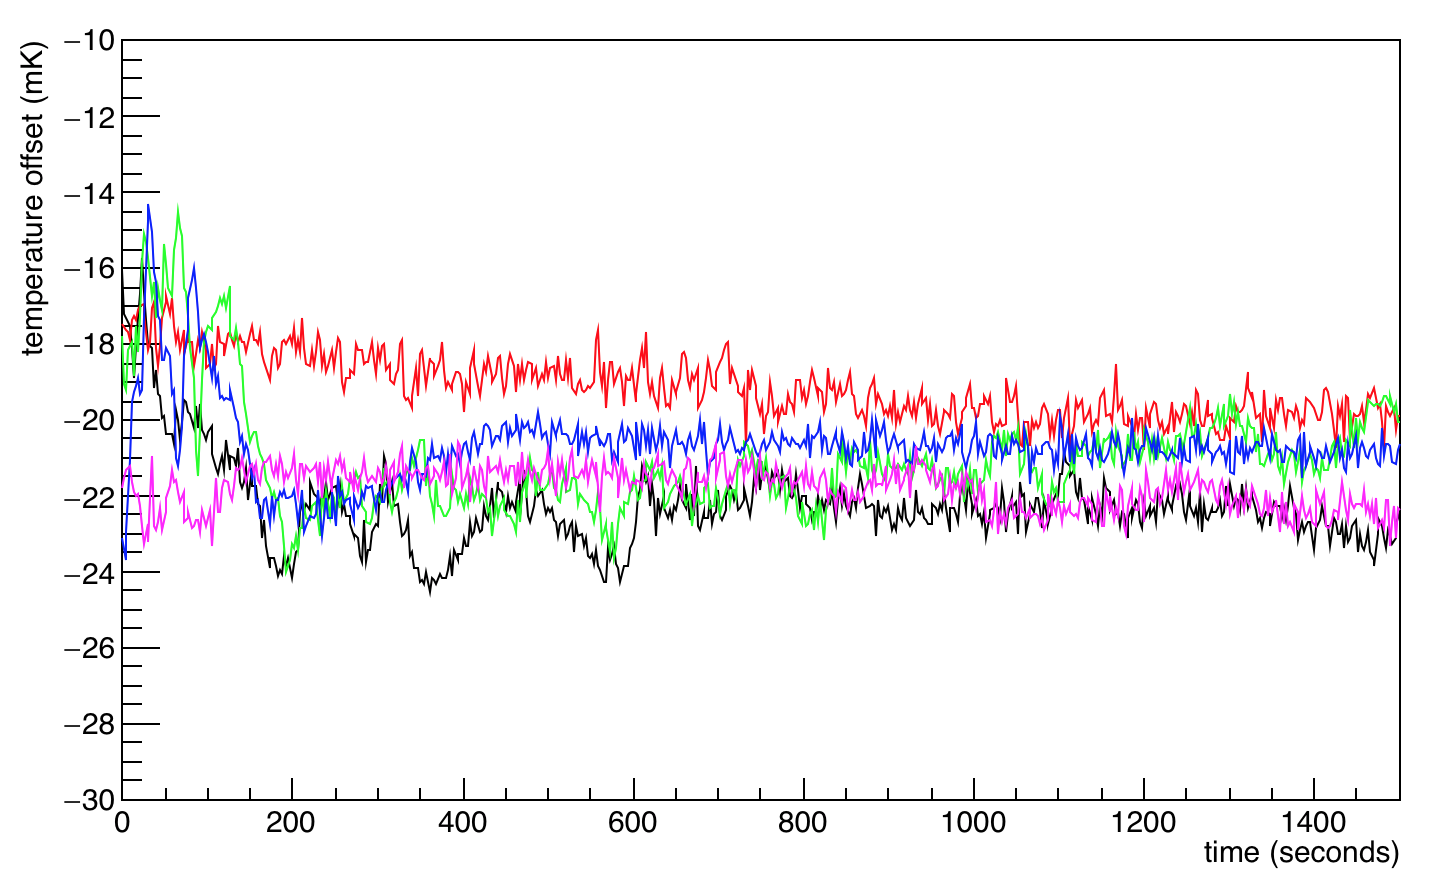
\includegraphics[width=0.5\textwidth]{cisc_Treproducibility.png}%
\end{dunefigure}


% % % %
\subsubsection{Dynamic T-gradient Monitors}

Dynamic temperature monitor is a vertical array of high precision temperature sensors with the goal of measuring vertical temperature gradient with precision of few \si{mK}. The design of the system is driven by two factors:
\begin{itemize}
\item
A few-\si{mK} uncertainty in the measured vertical temperature profile over the entire detector height is required in order to monitor \lar purity and provide useful feedback of efficiency of cryogenic recirculation and purification.
\item
Simulations of the cryogenic recirculation predict very slow change in temperature at meter scale except at the bottom and top of the cryostat. Thus, sensors are placed every \SI{50}{cm} along the \dword{detmodule} height with increased frequency in the first \SI{50}{cm}, closest to the bottom of the cryostat and the last \SI{50}{cm}, closest to the top of the cryostat, where spacing between sensors is reduced to \SI{10}{cm}.
 \end{itemize}


% In order to address concerns related to potential difference in the sensor reading prior to %installation 
% and after installation in a \dword{detmodule}, a dynamic temperature monitor allows cross-calibration of sensors in situ. Namely, this T-gradient monitor  can move vertically while installed in \dword{detmodule}, which allows for precise cross-calibration between the sensors in-situ at predefined locations, as well as in between them. The procedure for cross-calibrations is the following: the temperature reading is taken at the lowest position with all sensors. The stepper motor then moves the carrier rod up for \SI{50}{cm} putting all sensors in the location of their neighbor that is \SI{50}{cm} above them. Then the second reading is taken. In this manner, except for the lowest position we have temperature measurement at each location with two adjacent sensors, and by linking the temperature offsets between the two readings at each location, temperature readings from all sensors are cross-calibrated in situ, cancelling all offsets due to electromagnetic noise or any parasitic resistances that may have prevailed despite the four point connection to the sensors that should cancel most of the offsets. These measurements are taken with very stable current source, which ensures high precision of repeated temperature measurements over time. The motion of the dynamic T-monitor is stepper motor operated, delivering measurements with high spatial resolution. 

%%anne to here saturday 4/27
 
 In order to address concerns related to potential difference in the sensor reading prior to %installation 
 and after installation in a \dword{detmodule}, a dynamic temperature monitor allows cross-calibration of sensors in situ. 
 \fixme{difference in voltage, or differences in the sensor reading that may happen? I think the latter... (anne)}
 Namely, this T-gradient monitor  can move vertically while installed in the \dword{detmodule}, which allows for precise cross-calibration between the sensors in situ at predefined locations, as well as in between them. \fixme{not clear}
 The procedure for cross-calibrations is the following: the temperature reading is taken at the lowest position with all sensors. The stepper motor then moves the carrier rod up for \SI{50}{cm} 
 \fixme{just ``up 50cm''?} putting all sensors in the location of their neighbor that is \SI{50}{cm} above them. 
 Then the second reading is taken. In this manner, except for the lowest position we have temperature measurement at each location with two adjacent sensors, and by linking the temperature offsets between the two readings at each location, temperature readings from all sensors are cross-calibrated in situ, cancelling all offsets due to electromagnetic noise or any parasitic resistances that may have prevailed despite the four point connection to the sensors that should cancel most of the offsets. These measurements are taken with very stable current source, which ensures high precision of repeated temperature measurements over time. The motion of the dynamic T-monitor is stepper motor operated, 
delivering measurements with high spatial resolution. \fixme{or spatial precision?}
 \fixme{above pgraph needs some work}


\subsubsection{Dynamic T-gradient Monitor Design}
%Dynamic T-gradient monitor consists of three distinct parts: carrier rod on which sensors are mounted, enclosure above the cryostat housing the space that allows vertical motion of the carrier rod 1.5\,m above its lowest location, and motion mechanism. The motion mechanism consists of a stepper motor connected to a gear and pinion motion mechanism through ferrofluidic dynamic seal. The sensors have two pins that are soldered to a printed circuit board (PCB). Two wires are soldered to the common soldering pad for each pin, individually.   There is a cutout in the PCB around the sensor that allows free flow of argon for more accurate temperature reading.  Stepper motors typically have very fine steps allowing high precision positioning of the sensors.  Figure~\ref{fig:fd-slow-cryo-dt-monitor-overview} shows the overall design of the dynamic T-gradient monitor with the sensor carrier rod, enclosure above the cryostat and stepper motor mounted on the side of the enclosure. The enclosure consists of two parts connected by 6-cross flange. One side of the 6-cross flange will be used to for the signal wires, another side will be used as a viewing window, while the two other ports will be spares. Figure~\ref{fig:fd-slow-cryo-sensor-mount}-Left shows the mounting of the PCB board on the carrier rod and mounting on the sensor on the PCB along with the four point connection to the signal readout wires. Finally, Figure~\ref{fig:fd-slow-cryo-sensor-mount}-Right shows the stepper motor mounted on the side of the rod enclosure. The motor is kept outside, at room temperature and its power and control cables are also kept outside.

A dynamic T-gradient monitor consists of three distinct parts: a carrier rod on which sensors are mounted, an enclosure above the cryostat housing the space that allows vertical motion of the carrier rod 1.5\,m above its lowest location, and motion mechanism. The motion mechanism consists of a stepper motor connected to a gear and pinion motion mechanism through ferrofluidic dynamic seal. The sensors have two pins that are soldered to a printed circuit board (PCB). Two wires are soldered to the common soldering pad for each pin, individually.   There is a cutout in the PCB around the sensor that allows free flow of argon for more accurate temperature reading.  Stepper motors typically have very fine steps allowing high-precision positioning of the sensors.  Figure~\ref{fig:fd-slow-cryo-dt-monitor-overview} shows the overall design of the dynamic T-gradient monitor with the sensor carrier rod, enclosure above the cryostat and stepper motor mounted on the side of the enclosure. The enclosure consists of two parts connected by 6-cross flange. One side of the 6-cross flange 
\fixme{is this one flange with six ``crosses'' or six ``cross flanges''?} are used to for the signal wires, another side are used as a viewing window, while the two other ports are spares. Figure~\ref{fig:fd-slow-cryo-sensor-mount}-Left shows the mounting of the PCB board on the carrier rod and mounting on the sensor on the PCB along with the four point connection to the signal readout wires. Finally, Figure~\ref{fig:fd-slow-cryo-sensor-mount}-Right shows the stepper motor mounted on the side of the rod enclosure. The motor is kept outside, at room temperature and its power and control cables are also kept outside.
 \fixme{above pgraph needs some work}

\begin{dunefigure}[Dynamic T-gradient monitor overview]{fig:fd-slow-cryo-dt-monitor-overview}
  {An overview of the dynamic T-gradient monitor.}
 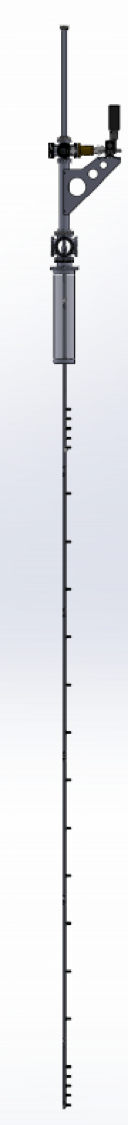
\includegraphics[width=0.11\textwidth,angle=90]{cisc_DTOverview.png}
\end{dunefigure}
\begin{dunefigure}[Sensor-cable assembly for dynamic T-gradient monitor]{fig:fd-slow-cryo-sensor-mount}
  {Left: Sensor mounted on a PCB board and PCB board mounted on the rod. Right:
    The driving mechanism of the dynamic T-gradient monitor. It consists of a stepper motor driving the pinion and gear linear motion mechanism. }
  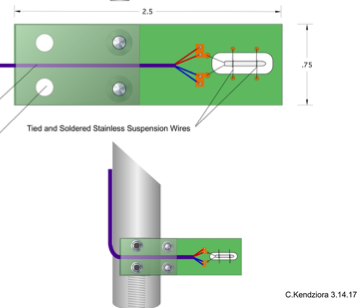
\includegraphics[width=0.40\textwidth]{cisc_DTSensorMount.png}
  \hspace{3cm}%
  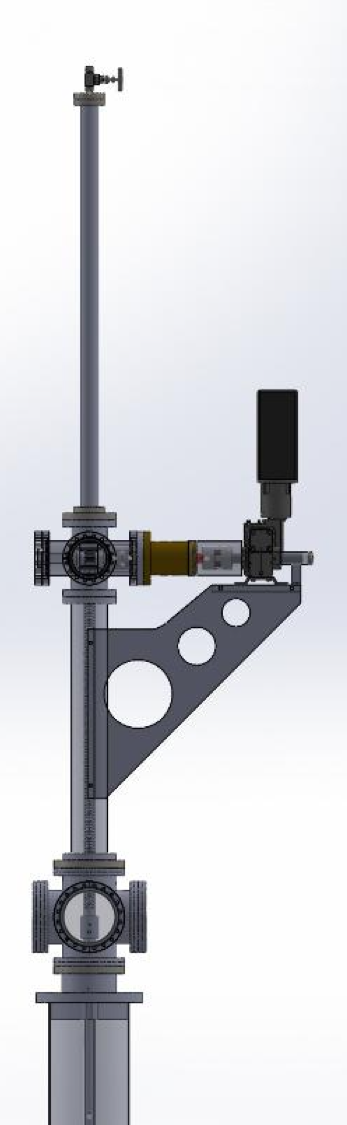
\includegraphics[width=0.12\textwidth]{cisc_DTMotor.png}
\end{dunefigure}

% % % %
\subsubsection{Individual Temperature Sensors}

T-Gradient monitors provide a vertical temperature profiling outside the TPCs. They are complemented by a coarser \twod array at the top and bottom of the
detector. Sensors, cables and readout system are the same as for the T-gradient monitors. 

In principle, a similar distribution of sensors is used at top and bottom.
Following the \dword{pdsp} design, bottom sensors use the cryogenic pipes as a support structure, while top sensors are anchored to the \dwords{gp}.
Teflon pieces (see Figure~\ref{fig:cable-support}) are used to route cables from the sensors to the CF63 side ports on \dword{dss}-cryogenics ports, which are used to extract the cables.
The PCB sensor's support, cables and connection to the flanges are the same as for the static T-gradient monitors. 

\begin{dunefigure}[Cable supports for individual temperature sensors]{fig:cable-support}
  {Left: support for two cables on ground planes. Right: Supports for three cables  mounted on cryogenics pipes using split clamps}
% This PDF is made from the .dot of the same name.
  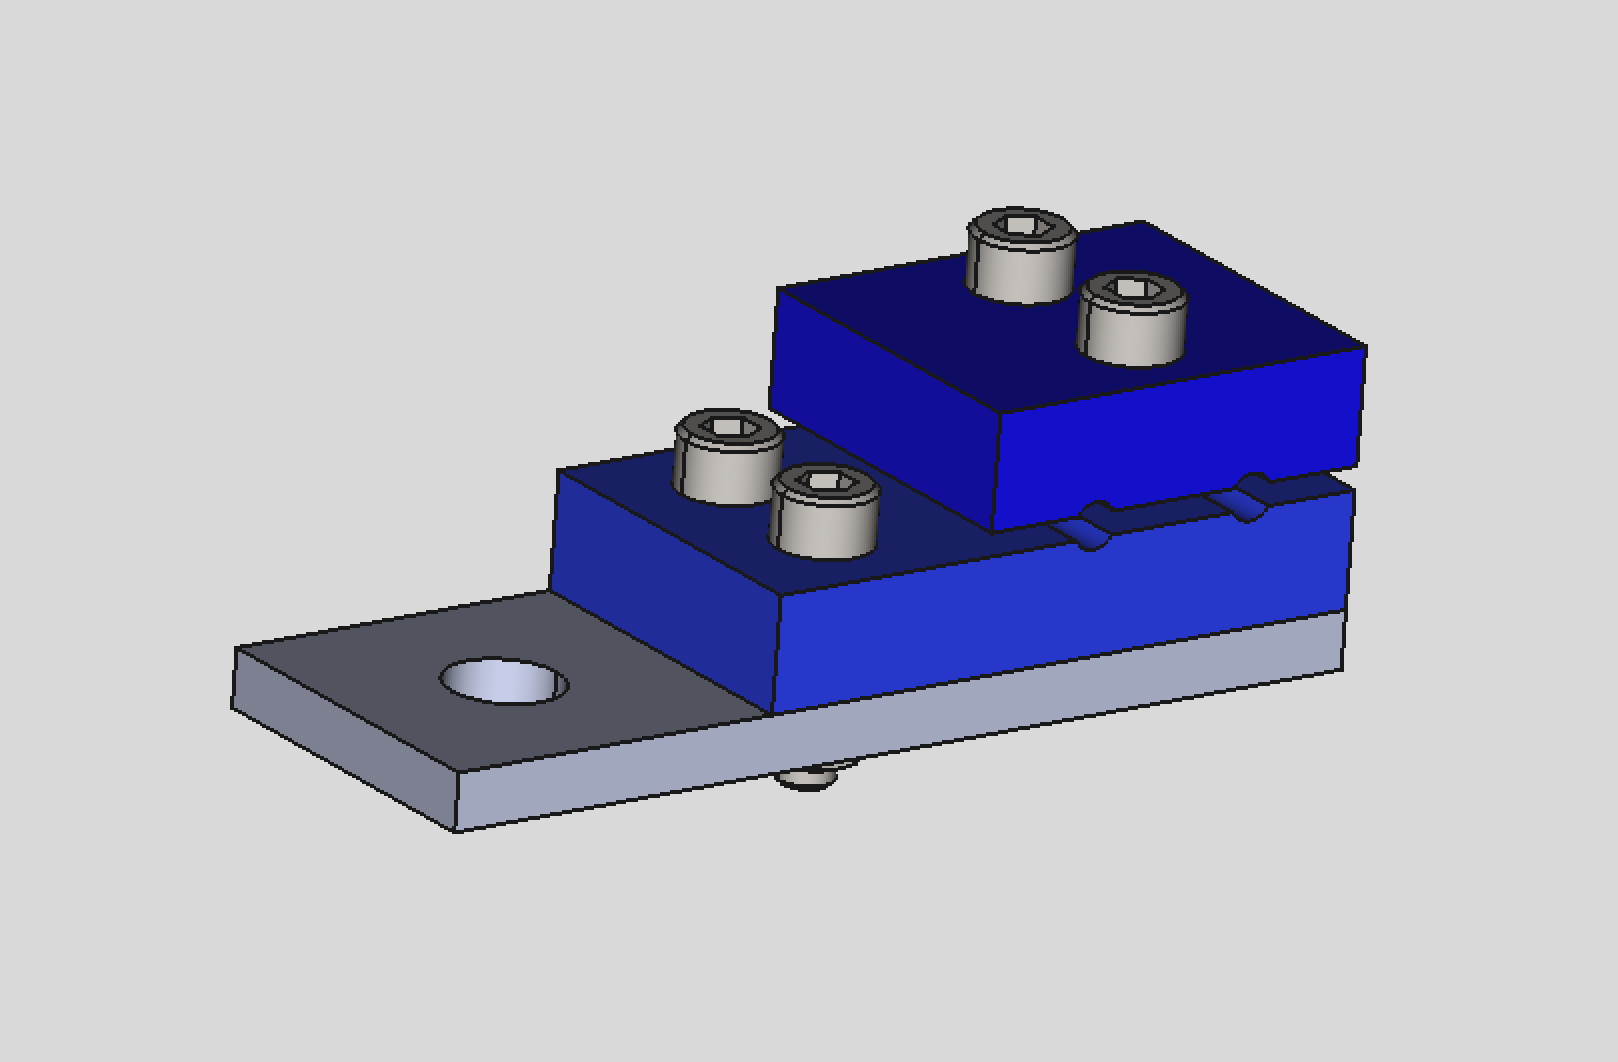
\includegraphics[width=0.3\textwidth]{cisc_TcableSupportGP.png}
  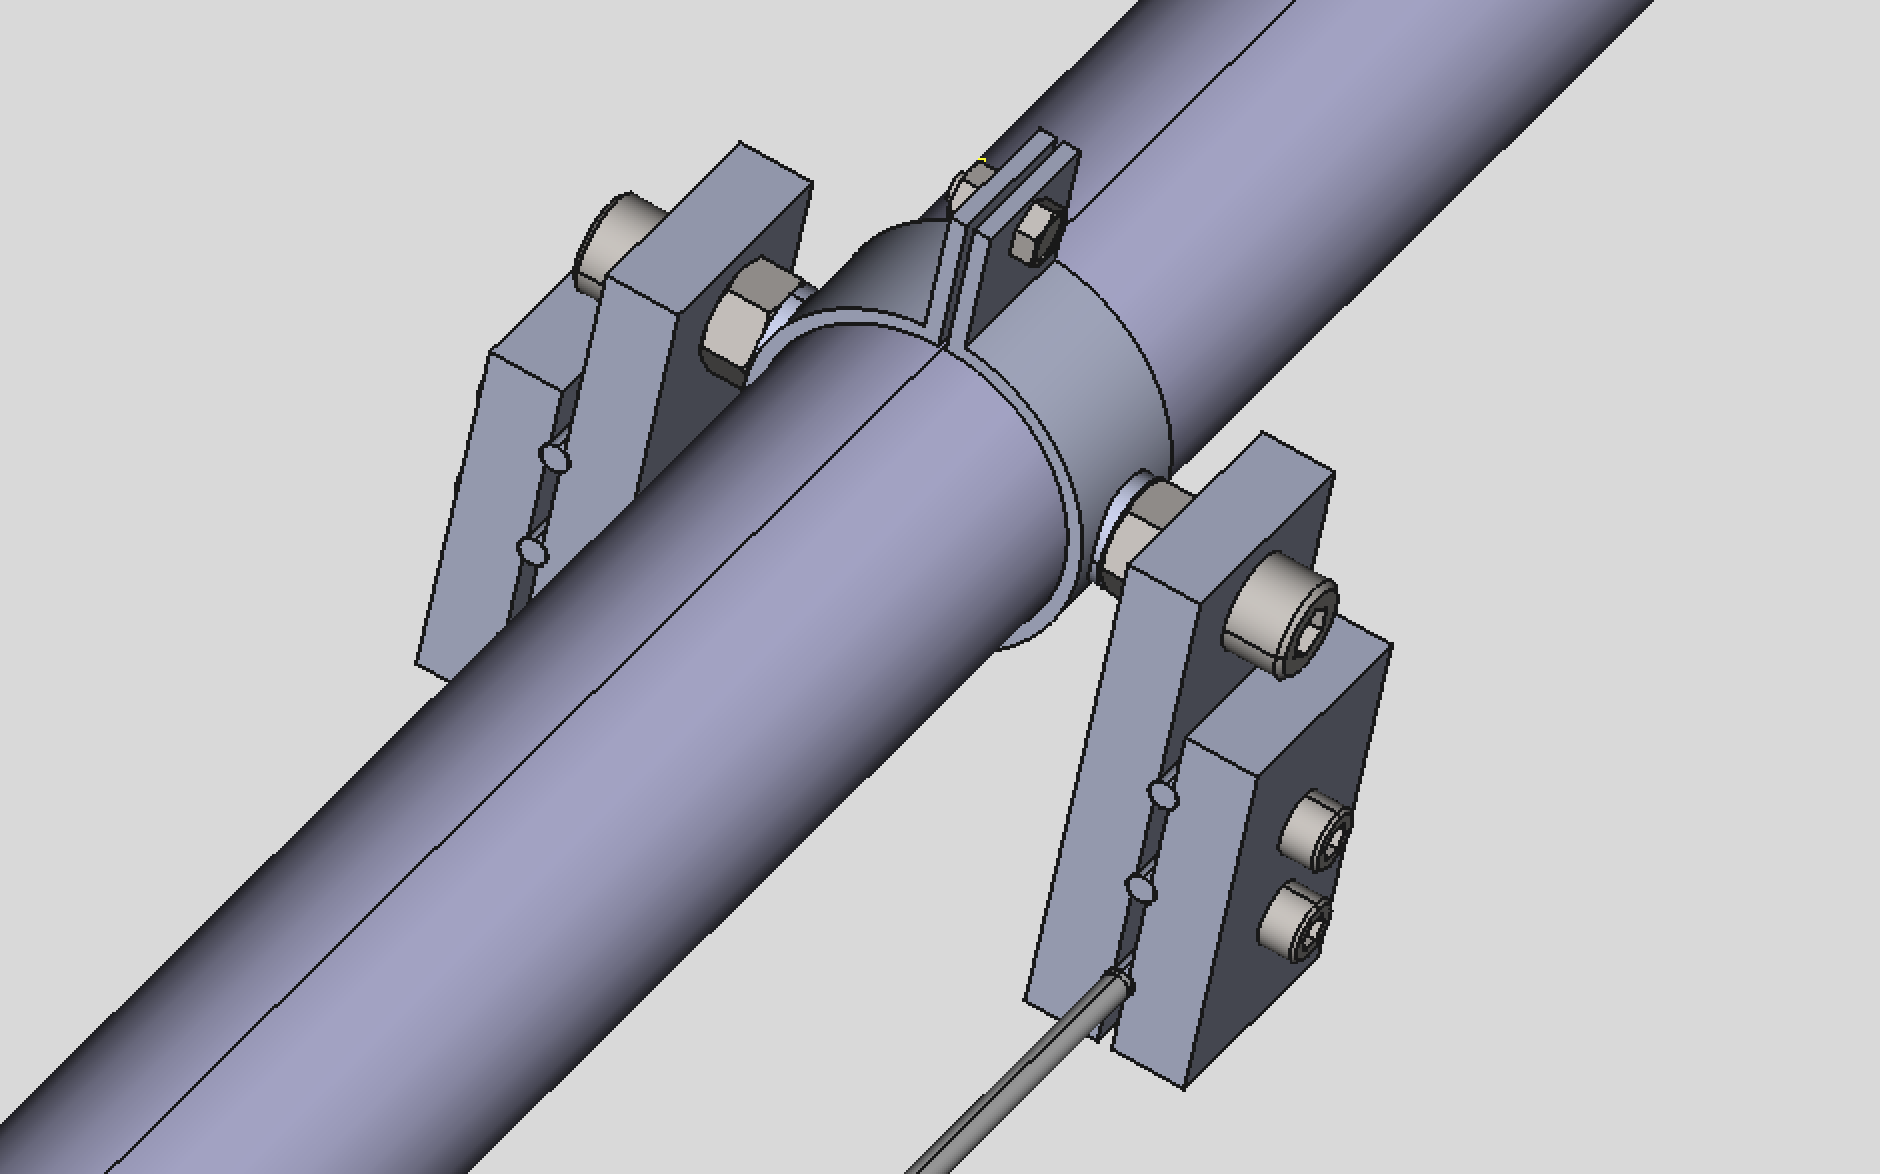
\includegraphics[width=0.315\textwidth]{cisc_TcableSupportPipes.png}
\end{dunefigure}


% % % %
\subsubsection{Readout System for Thermometers}
\label{sec:fdgen-slow-cryo-therm-readout}

A high precision and very stable system is required to achieved the design precision of $<\SI{5}{mK}$.
The proposed readout system is the one used in \dword{pdsp}, which is based on a variant of an existing mass PT100 temperature readout system developed at
CERN for one of the LHC experiments. The system consists of three parts:
\begin{itemize}
\item An accurate current source for the excitation of the temperature sensors, implemented by a compact electronic circuit using a high-precision voltage reference from Texas Instruments~\footnote{Texas Instruments\texttrademark{}, \url{http://www.ti.com/}.};
\item A multiplexing circuit based on an ADG707 Analog Device multiplexer electronic device;
\item A high-resolution and accuracy voltage signal readout module based on National Instruments~\footnote{National Instruments\texttrademark{}, \url{http://www.ni.com/en-us.html/}.} NI9238, which has \SI{24}{bit} resolution over a \SI{1}{V} range.
  This module is inserted in a National Instruments compact RIO device that distributes the temperature values to the main slow control software
  through the standard protocol, OPC UA. The Ethernet \dword{daq} also includes the multiplexing logic.
\end{itemize}


The current mode of operation averages over \num{2000} samples taken every second for each sensor. 
As inferred from Figure~\ref{fig:Trepro} the system has a resolution better than
\SI{1}{mK}, the \rms of one of the offsets in the stable region.

